% siminos/atlas/slice.tex  pdflatex atlas
% $Author$ $Date$


\section{Reduction of continuous symmetry}
\label{s:slice}

\subsection{The 3 ideas}

 Hilbert

 method of connections

 \mslices

    \begin{itemize}
      \item closest point on a group orbit
      \item variation $\to$ \slice\ hyperplane
    \end{itemize}

\subsection{Norms - distances between states}

We have seen that in presence of the continuous $\SOn{2}$ symmetry
\reqva\ and \rpo s are 2- and 3-dimensional manifolds of physically
equivalent states. How are we to compare a pair of such states? We shall
do this here by determining the minimal distance between them.

%%%%%%%%%%%%%%%%%%%%%%%%%%%%%%%%%%%%%%%%%%%%%%%%%
% 2011-08-23 Predrag: replaces BeThTraj.pdf from
% dasbuch/book/FigSrc/inkscape/BeThTraj.svg
% 2011-09-09 Predrag: updated
%            continuous.tex overheads, and ChaosBook
\begin{figure}
 \begin{center}
  \setlength{\unitlength}{0.20\textwidth}
  %% \unitlength = units used in the Picture Environment
(a)~~
  \begin{picture}(1,1.07471658)%
    \put(0,0){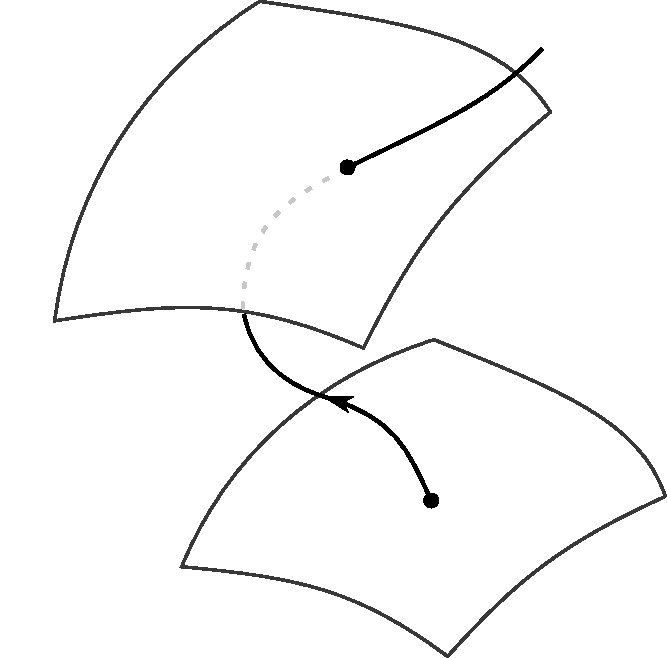
\includegraphics[width=\unitlength]{BeThTrajTeX}}%
    \put(0.28879298,1.02196543){\color[rgb]{0,0,0}\rotatebox{-22.37140782}{\makebox(0,0)[lb]{\smash{$\pS_{\ssp(\zeit)}$}}}}%
    \put(0.55566402,0.45078735){\color[rgb]{0,0,0}\rotatebox{-16.6673442}{\makebox(0,0)[lb]{\smash{$\pS_{\ssp(0)}$}}}}%
    \put(0.63028127,0.18433597){\color[rgb]{0,0,0}\rotatebox{0.03136739}{\makebox(0,0)[lb]{\smash{$\ssp(0)$}}}}%
    \put(0.46253394,0.70182304){\color[rgb]{0,0,0}\rotatebox{0.03136739}{\makebox(0,0)[lb]{\smash{$\ssp(\zeit)$}}}}%
    \put(0.03852492,0.09250899){\color[rgb]{0,0,0}\rotatebox{0.11031334}{\makebox(0,0)[lb]{\smash{$\pS$}}}}%
  \end{picture}%
~~(b)
  \begin{picture}(1,1.07315413)%
    \put(0,0){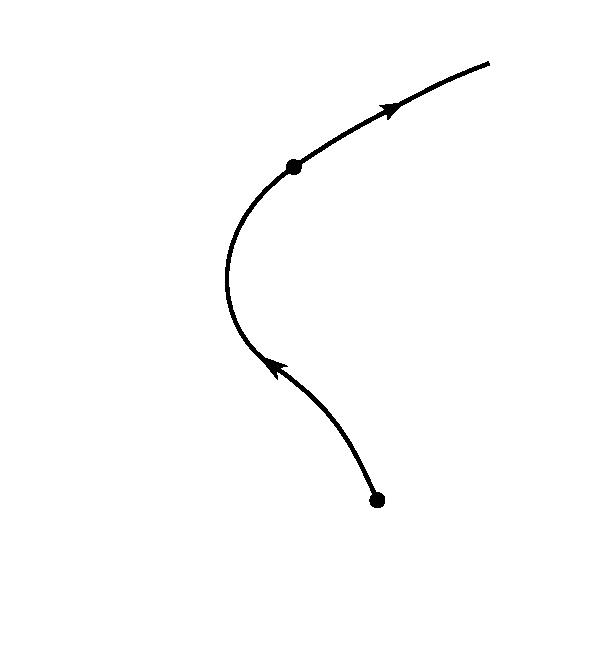
\includegraphics[width=\unitlength]{BeThRedTeX}}%
    \put(0.19912369,0.17144733){\color[rgb]{0,0,0}\rotatebox{0.11031334}{\makebox(0,0)[lb]{\smash{$\pSRed$}}}}%
    \put(0.63028127,0.18433598){\color[rgb]{0,0,0}\rotatebox{0.03136739}{\makebox(0,0)[lb]{\smash{$\sspRed(0)$}}}}%
    \put(0.46253394,0.70182305){\color[rgb]{0,0,0}\rotatebox{0.03136739}{\makebox(0,0)[lb]{\smash{$\sspRed(\zeit)$}}}}%
  \end{picture}%
 \end{center}
% (a) 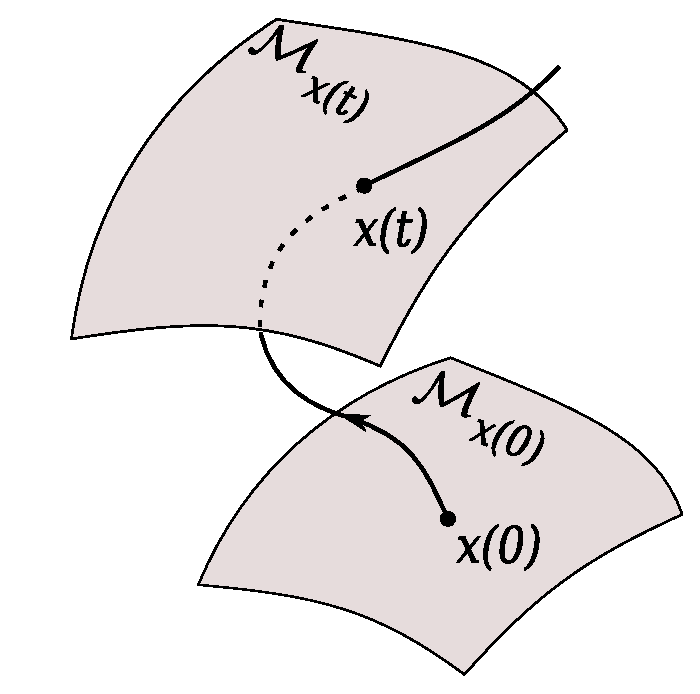
\includegraphics[width=0.45\textwidth]{BeThTraj}
  \caption{\label{fig:BeThTraj}
(a)
The group orbit $\pS_{\ssp(0)}$ of \statesp\ point $\ssp(0)$, and the
group orbit $\pS_{\ssp(\zeit)}$ reached by the trajectory $\ssp(\zeit)$ time $t$
later.
(b)
Symmetry reduction $\pS \to \pSRed$ replaces each full \statesp\
group orbit $\pS_{\ssp}\subset\pS$ by a single point $\sspRed \in \pSRed$.
  }
\end{figure}
%%%%%%%%%%%%%%%%%%%%%%%%%%%%%%%%%%%%%%%%%%%%%%%%%%

\begin{figure}
  \centering
(a) ???~~~~
(b)%\includegraphics[width=0.45\textwidth]{2840GOt135th0}
  \caption{\label{fig:2840GOt135th0}
    %\label{fig:M1groupOrb}
Projections of group orbits of two states $\ssp$ (in $\approx
100,000$-dimensional {\statesp}) onto a stationary Frenet-Serret frame
given by unit vectors in the directions
$\{\groupTan_z(\ssp'),\groupTan_\theta(\ssp'),\normVec_z(\ssp')\}$ (see
\refeq{FrenetFrame}). The group orbit is generated by
$\LieEl(0,\shift)\,\ssp$, i.e. by axial shifts, and plotted relative to the
point $\ssp'$.
In  (b) $\ssp$ is a strongly nonlinear chaotic state.
Group orbits are only topologically circles, and inflections are possible
when $\ssp$ is not so close to $\ssp'$.
%{APW 111027 For N2_UB, only see mild distortions;
% see fig 15(b) of dailyBlog}
  }
\end{figure}


\begin{figure}
  \centering
(a)%\includegraphics[width=0.45\textwidth]{2839GOLB}
(b)%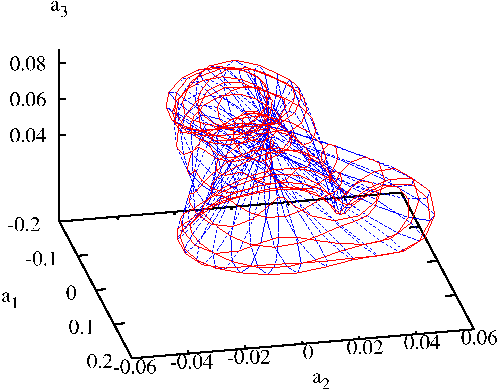
\includegraphics[width=0.45\textwidth]{2840GOt135M1}
  \caption{\label{fig:2830GO6}
    %\label{fig:M1groupOrb}
As \reffig{fig:2840GOt135th0}, but with the
full 2\dmn\ $\SOn{2}_{\theta} \times \SOn{2}_z$ group orbits traced out
by shifts in both $z$ and $\theta$. Loops in solid red correspond to
shifts in $z$, dashed blue loops to shifts in $\theta$.
%(a) \Reqv\ N2\_LB, (b) \Reqv\ N2\_UB.
  }
\end{figure}

\subsection{The goal, 3 ideas}

The goal of \emph{symmetry reduction} is to replace each group orbit by a
unique point in a lower-dimensional symmetry-\reducedsp\ $\pSRed =
\pS/\Group$, as sketched in \reffig{fig:BeThTraj}. Several symmetry
reduction schemes are reviewed in \refref{SiCvi10}. Here we shall
describe the \mslices\rf{rowley_reconstruction_2000,BeTh04,FrCv11}, the
only method that we find practical for a symmetry reduction of
chaotic solutions of highly nonlinear flows, see \refsect{s:rpos}.

In the \mslices\ the symmetry reduction is achieved by cutting the group
orbits with a finite set of hyperplanes, one for each continuous group
parameter, with each group orbit of
symmetry-equivalent points represented by a single point, its
intersection with the \slice.
The procedure is akin to (but distinct from)
cutting across continuous-time parametrized trajectories by
means of Poincar\'e sections.
    \PC{``
        analogous to the way a \PoincSec\ reduces a continuous time orbit
        to a sequence of points. It should be noted, however, that a
        \slice\ is \emph{not} a \PoincSec.
    ''}
As is the case for Poincar\'e sections,
choosing a `good' \slice\ is a dark art. Our guiding principle is to chose
a \slice\ such that the distance between a `{\template}' state {\slicep} and nearby
group orbits is \emph{minimized}, \ie, identify the point $\sspRed$ on the group
orbit \refeq{sspOrbit} of a nearby state $\ssp$ which is the closest
match to the {\template} point {\slicep}.


\subsection{\Mslices; a local chart}

After some experimentation and observations of turbulence in a given
flow, one can identify a set of dynamically important unstable
{\recurrStr s}.
    \PC{refer to \refsect{s:cut}}

We shall refer to this catalogue of $m$ representative snapshots
or `reference states', either precomputed or
experimentally measured, as  \emph{\template s}
\rf{rowley_reconstruction_2000}, each an instantaneous state of the
$3D$ fluid flow represented by a
\emph{point} $\slicep{}^{(j)}$, $j=1,2,\cdots,m$, in the
\statesp\ $\pS$ of the system. The symmetries of the flow (i.e.\ the
$\LieEl\in\Group$) are then used to shift and rotate the {\template}
$\slicep$ until it overlies, as well as possible, the {\cohStr} of
interest $\ssp$, by minimising the distance
\beq
\Norm{\ssp - \LieEl(\gSpace)\,\slicep}
%    = \Norm{\LieEl(-\gSpace)\,\ssp - \slicep}
%    = \Norm{\sspRed - \slicep}
\, .
\ee{minDistance}
The entire group orbit of $\ssp$ is then replaced
by the closest match to
the {\template} pattern,
given by
$\sspRed=\LieEl^{-1}\ssp$, %=\LieEl(-\gSpace)\ssp$,
as shifting does not affect the norm,
$\Norm{\ssp-\LieEl\,\slicep}=\Norm{\sspRed-\slicep}$.
The symmetry \reducedsp\ $\pSRed$, of dimension $(d\!-\!1)$, consists of
the set of closest matches $\sspRed$, one element for each full \statesp\ $\pS$
group orbit; the bar on $\sspRed$
indicates the unique point on the group orbit of $\ssp$ closest to
the \template\ \slicep.

For the reduction of a
$\SOn{2}$ symmetry, the minimal distance satisfies the extremum
condition
    \PC{make 2 lines?}
\[
\frac{\partial}{\partial \gSpace} \Norm{\ssp - \LieEl(\gSpace)\,\slicep}^2
   =
2\, \braket{\ssp - \LieEl\,\slicep}{\Lg_\gSpace \,\LieEl\,\slicep}
   =
2\, \braket{\sspRed - \slicep}{\Lg_\gSpace \slicep}
   = 0
    \, ,
\]
given that group orbits are smooth differentiable manifolds.
As $\Norm{\LieEl(\gSpace)\slicep}$ is a constant,
the group tangent vector $\Lg_\gSpace \slicep$
evaluated at $\slicep$
\refeq{eq:tang} %GroupTangField}
is normal to $\slicep$, and
the term $\braket{\slicep}{\Lg_\theta\,\slicep}$ vanishes
($\Lg_{\theta}$ is antisymmetric).
Therefore the point $\sspRed$ on the group
orbit that lands in the \slice, satisfies the \emph{\slice\ condition}
\beq
\braket{\sspRed}{\sliceTan{\theta}} = 0
    \,,\quad
\sliceTan{\theta} = \Lg_\theta \slicep
    \,.
\ee{PCsectQ0}
The \slice\ so defined is therefore
a hyperplane that includes the origin,
normal to the \template\ group tangent %$\sliceTan{\theta}$
evaluated at the \template.

%%%%%%%%%%%%%%%%%%%%%%%%%%%%%%%%%%%%%%%%%%%%%%%%%%%%%%%%%%%%%%%%
%% slice.*, inflectHype.*: see dasbuch/book/FigSrc/inkscape/00ReadMe.txt
%% rpo.* hand-drawn in dasbuch/book/FigSrc/xfig/rpo.fig
%% xfig exported -> FigSrc/inkscape/rpo.fig
%% inkscape exported -> rpo.eps + LaTeX, hand edited in the macros
%% Predrag 2011-08-27 replaced rpo.pdf by rpoSlice.pdf
%% remember to insert rpoSlice.pdf into ChaosBook

 \begin{figure}
 \begin{center}
  \setlength{\unitlength}{0.20\textwidth}
  %% \unitlength = units used in the Picture Environment
(a)
  \begin{picture}(1,0.87085079)%
    \put(0,0){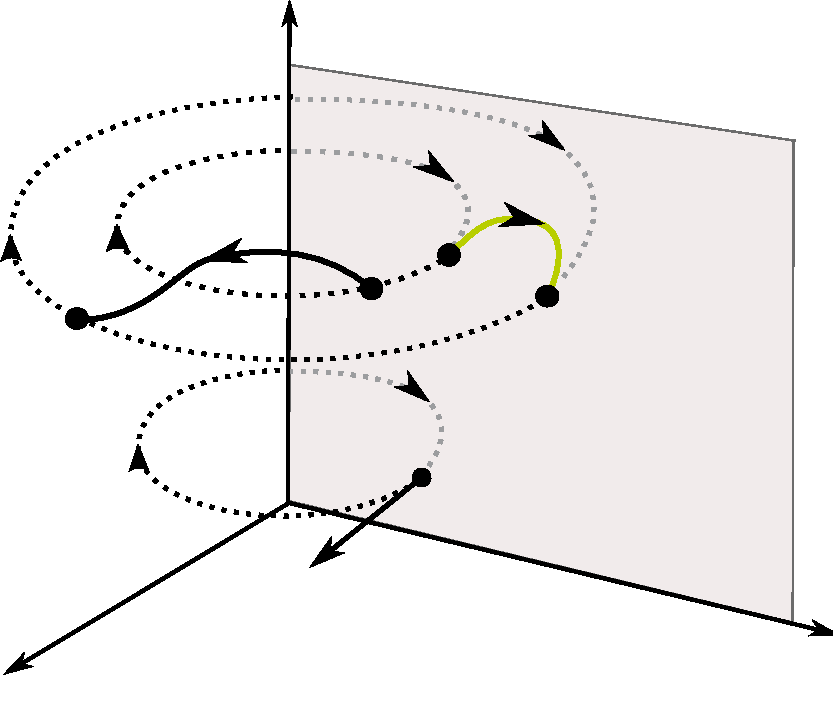
\includegraphics[width=\unitlength]{slice}}%
    \put(0.82835155,0.19007659){\color[rgb]{0,0,0}\rotatebox{-14.84025424}{\makebox(0,0)[lb]{\smash{$\pSRed$}}}}%
    \put(0.07077338,0.28688228){\color[rgb]{0,0,0}\rotatebox{0.0313674}{\makebox(0,0)[lb]{\smash{$\LieEl\,\slicep$}}}}%
    \put(0.53023327,0.26593335){\color[rgb]{0,0,0}\rotatebox{0.0313674}{\makebox(0,0)[lb]{\smash{$\slicep$}}}}%
    \put(0.4284954,0.179285){\color[rgb]{0,0,0}\rotatebox{0.0313674}{\makebox(0,0)[lb]{\smash{$\sliceTan{}$}}}}%
    \put(0.00798985,0.42305068){\color[rgb]{0,0,0}\rotatebox{0.0313674}{\makebox(0,0)[lb]{\smash{$\ssp(\zeit)$}}}}%
    \put(0.65766235,0.45412105){\color[rgb]{0,0,0}\rotatebox{0.0313674}{\makebox(0,0)[lb]{\smash{$\sspRed(\zeit)$}}}}%
    \put(0.06916446,0.74280851){\color[rgb]{0,0,0}\rotatebox{0.0313674}{\makebox(0,0)[lb]{\smash{$\LieEl(\zeit)$}}}}%
  \end{picture}%
~~~
(b)
  \begin{picture}(1,0.87085079)%
    \put(0,0){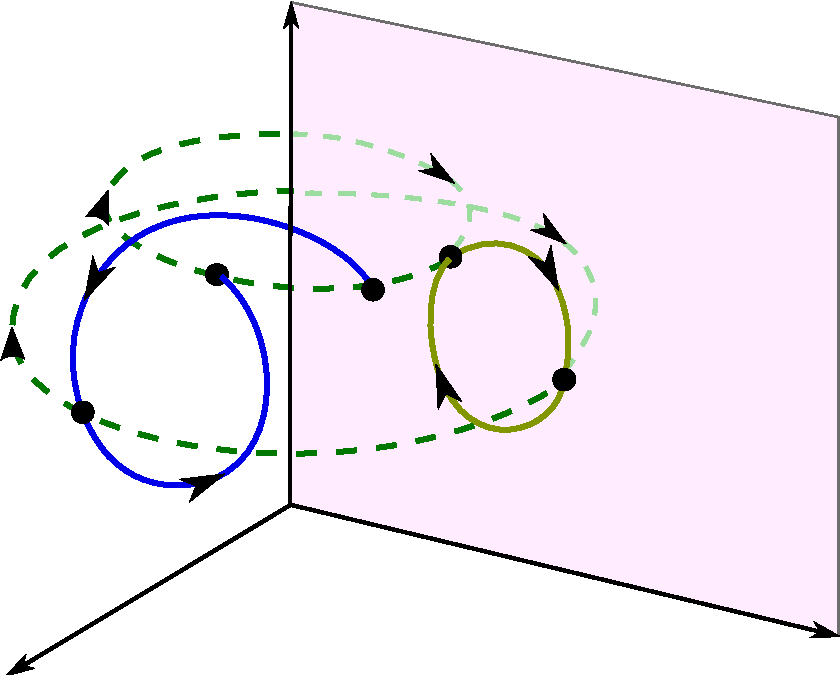
\includegraphics[width=\unitlength]{rpoSlice}}%
    \put(0.82835153,0.19007656){\color[rgb]{0,0,0}\rotatebox{-14.84025432}{\makebox(0,0)[lb]{$\pSRed$}}}%
    \put(0.40925459,0.45713857){\color[rgb]{0,0,0}\rotatebox{0.0313674}{\makebox(0,0)[lb]{\smash{$\ssp(0)$}}}}%
    \put(0.71354118,0.39765314){\color[rgb]{0,0,0}\rotatebox{0.0313674}{\makebox(0,0)[lb]{\smash{$\sspRed(\zeit)$}}}}%
    \put(0.13171187,0.38813817){\color[rgb]{0,0,0}\rotatebox{0.0313674}{\makebox(0,0)[lb]{\smash{$\LieEl(\zeit)$}}}}%
    \put(0.02168739,0.31359574){\color[rgb]{0,0,0}\rotatebox{0.0313674}{\makebox(0,0)[lb]{\smash{$\ssp(\zeit)$}}}}%
    \put(0.15576193,0.48769256){\color[rgb]{0,0,0}\rotatebox{0.0313674}{\makebox(0,0)[lb]{\smash{$\ssp(\period{})$}}}}%
    \put(0.54113911,0.50476963){\color[rgb]{0,0,0}\rotatebox{0.0313674}{\makebox(0,0)[lb]{\smash{$\sspRed(0)$}}}}%
  \end{picture}%
 \end{center}
 \caption{\label{fig:slice}
The \mslices, a \statesp\ visualization:
(a)
\Slice\ $\pSRed \supset \pS/\Group$ lies in the $(d\!-\!N)$\dmn\
hyperplane \refeq{PCsectQ0} normal to $\sliceTan{}$, where $\sliceTan{j}$
span the  $N$\dmn\ space tangent to the group orbit $\LieEl\,\slicep$
(dotted line) evaluated at the {\template} point $\slicep$. The
hyperplane intersects {\em all} full \statesp\ group orbits (green
dashes). The full \statesp\ trajectory $\ssp(\zeit)$ (blue) and the
\reducedsp\ trajectory $\sspRed(\zeit)$ (green) are equivalent up to a
`moving frame' rotation $\ssp(\zeit)=\LieEl(\zeit)\,\sspRed(\zeit)$, where
$\LieEl(\zeit)$ is a shorthand for $\LieEl(\gSpace(\zeit))$.
(b)
In the full \statesp\ $\pS$ a \rpo\ $\ssp(0) \to \ssp(\zeit) \to
\ssp(\period{})$ returns to the group orbit of $\ssp(0)$ after time
$\period{}$ and a rotation by $\LieEl$,  $\ssp(0)=\LieEl \, \ssp
(\period{})$. For flows with continuous symmetry a generic \rpo\ fills
out quasi-\-periodically what is topologically a torus. In the \slice\
$\pSRed$ the symmetry-reduced orbit is periodic, $\sspRed(0) =
\sspRed(\period{})$. This is a highly idealized sketch: A group orbit is
a $N$\dmn\ manifold, and even for $\SOn{2}$ it is usually only
topologically a circle (see \reffig{fig:2840GOt135th0}), and can
intersect a hyperplane any number of times  (see \reffig{fig:sliceimage}).
 }
 \end{figure}


When $\ssp$ is varies in time, $\dot{\ssp}=\vel(\ssp)$,
the {\template} $\slicep$ tracks the motion
using the slice condition \refeq{PCsectQ0} to
minimise $\Norm{\ssp(\zeit)-\LieEl(\theta(\zeit))\slicep}$,
and the
full-space trajectory $\ssp(\zeit)$ is thus rotated into the {\reducedsp},
$\sspRed(\zeit) = \LieEl^{-1}\,\ssp(\zeit)$,
by appropriate
\emph{moving frame} angles $\{\gSpace(\zeit)\}$, as depicted in
\reffig{fig:slice}\,(a).
%
Specializing to $\SOn{2}$, one can write the
equations for the \reducedsp\
flow, $\sspRed(\zeit) \in \pSRed$,
confined to the \slice, $\dot{\sspRed} = \velRed(\sspRed)$,
as
\bea
\velRed(\sspRed) &=& \vel(\sspRed)
     \,-\, \dot{\gSpace}(\sspRed) \, \groupTan(\sspRed)
\label{EqMotMFrame}\\
\dot{\gSpace}(\sspRed) &=& \braket{\vel(\sspRed)}{\sliceTan{}}
                       /\braket{\groupTan(\sspRed)}{\sliceTan{}}
\,.
\label{reconstrEq}
\eea
In other words, $\vel$, the velocity in the full \statesp, can be written
as the sum of $\velRed$, the velocity component in the \slice, and
$\dot{\gSpace}\,\groupTan$, the Cartan derivative \refeq{CartanDer} or
the velocity component within the group tangent space. The
$\dot{\gSpace}$ equation is the {\em reconstruction equation}: its
integral keeps track of the group shifts in the full \statesp. In
particular, if  \sspRed\ is a point on a \reqv\ \refeq{phaseVel}, the full \statesp\
velocity equals the phase velocity, and $\velRed(\sspRed) = 0$, \ie,
\reqva\ are always reduced to \eqva\ in the \reducedsp. It should be
emphasized that we never integrate the reduced equations
\refeq{EqMotMFrame}; numerical simulations are always carried out in the
full \statesp. Slicing is implemented as postprocessing of numerical or
experimental data, by rotating full \statesp\ trajectories into the
\slice, as in \reffig{fig:sliceimage}.



\subsection{What it is not}
    \begin{itemize}
      \item comoving frame
      \item an average over the group phase variables
      \item reduced-dimensionality model
    \end{itemize}
